%INTENTO 1

%En el Capítulo \ref{cap:int} se detalló que el sisetma desarrollado se compone de tres componentes principales, a saber: El Host, cuyo rol es llevado a cabo por una PC; la interfaz, integrada por el controlador FX2LP de Cypress y un FPGA, en este caso un Spartan-6 de Xilinx. A su vez, el Capítulo \ref{cap:fpga}, indica que el sistema interno del FPGA lleva una Maquina de Estados Finitos (MEF), cuya función es la de realizar el efectivo intercambio de datos con la interfaz, y un sistema genérico.
%
%Hasta acá se ha desarrollado la configuración de la interfaz y la implementación de la MEF. Sin embargo, es necesario, que el sistema pueda funcionar en forma autónoma, proveerle un sistema mínimo que pueda hacer las veces de fuente y sumidero de datos. Es por esto, que se dotó al sistema con una memoria FIFO con el objetivo de implementar un eco que permita realizar una evaluación de desempeño de la comunicación desarrollada. Así, se permite enviar mensajes desde una PC y que estos sean recibidos luego.
%
%\subsection{Implementación de la memoria FIFO en el FPGA}
%	La memoria FIFO sintetizada en el FPGA se obtuvo a través de la herramienta {\it Core Generator} provista por Xilinx junto con el entorno de desarrollo ISE, utilizado en este trabajo para el desarrollo\cite{XilinxInc}. La configruación seleccionada generó una memoria FIFO de 511 bytes, con puertos de entrada y salida dedicados, es decir uno de entrada y uno de salida, un bus de 16 bits de ancho. Posee señal de reconocimiento de escritura. También se dotó a la memoria generada con entradas de reloj y habilitación de bus independientes tanto para el puerto de entrada como el puerto de salida.
%	
%	
%INTENTO 2
%TODO debería decir como generar cada una de las señales internas propuesas en el capitulo correspondiente... la magen en cuestion es \ref{fpga:intersignal}
%Con el objetivo de verificar el sistema desarrollado, se procedió a implementarlo en un sistema mínimo que sea capaz de utilizar la comunicación, de forma tal que el Host pueda establecer un enlace con el FPGA. Para ello, se implementó un sistema eco, es decir, un sistema que recibe los mensajes que envía el Host y, luego, los transmite para que el Host pueda recibirlos. De esta forma, el Host puede reconocer que los datos enviados no fueron perdidos ni modificados.

% INTENTO 3
El sistema desarrollado en el FPGA para realizar las pruebas de desempeño implementa la MEF desarrollada en el Capítulo \ref{cap:fpga}, debido a que es uno de los componentes principales en lo que a las pruebas se refieren. Sin embargo, el sistema también requiere de capacidad de almacenamiento de los datos que son provistos desde la PC y de una señal de reloj.

Para cubrir los requerimientos de capacidad de datos, se utiliza una memoria FIFO. Así, los datos que son enviados desde la PC, se almacenan en la memoria FIFO a medida que arriban, atravesando la interfaz. Luego, estos datos son reenviados desde la misma memoria FIFO, emprendiendo el circuito hacia la PC.

La señal de reloj del FPGA es provista por un oscilador incorporado en la placa de desarrollo Mojo v3. La señal de reloj a la frecuencia necesaria se obtiene adaptando la señal generada por el oscilador a través de un PLL.

Tanto el PLL como la memoria FIFO incorporadas al sistema implementado dentro del FPGA, fueron generadas por la herramienta \textit{Core Generator}, provista por la empresa Xilinx Inc. en el software de programación ISE.

\begin{figure}[t]
	\centering
	\begin{tikzpicture}[scale=.7]
		\begin{scope}[transform shape,node distance=4,>=latex,double distance=1.3]
			\node[simple](mea)[]{Maquina de Estados Finitos};
			
			\node[simple,rounded corners](fx2lp)[left=of mea]{Interfaz USB};
			\draw[<->,double]([yshift=10*220/11]fx2lp.south east) --node[above]{FD[15:0]}([yshift=220/11*10]mea.south west);
			\draw[<-,double]([yshift=220/11*9]fx2lp.south east) --node[above]{FADDR[1:0]}([yshift=220/11*9]mea.south west);
			\draw[->]([yshift=220/11*8]fx2lp.south east) --node[above]{FLAGA}([yshift=220/11*8]mea.south west);
			\draw[->]([yshift=220/11*7]fx2lp.south east) --node[above]{FLAGB}([yshift=220/11*7]mea.south west);
			\draw[->]([yshift=220/11*6]fx2lp.south east) --node[above]{FLAGC}([yshift=220/11*6]mea.south west);
			\draw[->]([yshift=220/11*5]fx2lp.south east) --node[above]{FLAGD}([yshift=220/11*5]mea.south west);
			\draw[->]([yshift=220/11*4]fx2lp.south east) --node[above]{SLWR}([yshift=220/11*4]mea.south west);
			\draw[->]([yshift=220/11*3]fx2lp.south east) --node[above]{SLRD}([yshift=220/11*3]mea.south west);
			\draw[->]([yshift=220/11*2]fx2lp.south east) --node[above]{SLOE}([yshift=220/11*2]mea.south west);
			\draw[->]([yshift=220/11*1]fx2lp.south east) --node[above]{PKTEND}([yshift=220/11*1]mea.south west);
			
			
			\node[simple,minimum height=150,minimum width=50](interno)[right=6 of mea.north east,anchor=north west]{Memoria FIFO};
			\draw[double,->]([yshift=-1*150/8]mea.north east)--node[above]{Dato\_enviado[15:0]} ([yshift=-1*150/8]interno.north west);
			\draw[double,<-]([yshift=-2*150/8]mea.north east)--node[above]{Dato\_a\_enviar[15:0]}([yshift=-2*150/8]interno.north west);
			\draw[<-]([yshift=-3*150/8]mea.north east)--node[above]{Enviar\_datos}([yshift=-3*150/8]interno.north west);
			\draw[<-]([yshift=-4*150/8]mea.north east)--node[above]{PKTEND}([yshift=-4*150/8]interno.north west);
			
			\node[simple,minimum height=70](adapt)[anchor=south] at  ($(mea.south|-interno.south)!0.5!(interno.south)$|-interno.south) {Adaptador};
			\draw[->]([yshift=-5.5*150/6]mea.north east)--node[above]{SLWR}([yshift=-5.5*150/6]mea.north east -| adapt.west);
			\draw[->]([yshift=-4.5*150/6]mea.north east)--node[above]{SLRD}([yshift=-4.5*150/6]mea.north east -| adapt.west);
			\draw[<-]([yshift=1*70/5]adapt.south east) --node[above]{Llena} ([yshift=1*70/5]adapt.south east -| interno.west);
			\draw[<-]([yshift=2*70/5]adapt.south east) --node[above]{Vacia} ([yshift=2*70/5]adapt.south east -| interno.west);
			\draw[->]([yshift=3*70/5]adapt.south east) --node[above]{wr\_en} ([yshift=3*70/5]adapt.south east -|interno.west);
			\draw[->]([yshift=4*70/5]adapt.south east) --node[above]{rd\_en} ([yshift=4*70/5]adapt.south east -|interno.west);
			
			\node[simple,minimum size=50](clk) [anchor=south]at (mea.south west-|interno.south)  {PLL};
			\draw[<-]([yshift=15]mea.east |- clk.west)--node[above,near end]{Reloj}([yshift=15]clk.west);
			\draw[->] (clk) -- node[right]{clk} (interno);
			\draw[->] ([yshift=15]clk.west) -| (adapt);
			
			\node[rounded corners,simple, minimum size=50](clkSrc)[right=1 of clk]{Fuente de reloj};
			\draw[->](clkSrc) to (clk);
			
			\node[simple,minimum size=30](rst)[anchor=south]at($(mea.south)!.5!(clk.south)$) {Reset};
			\draw[->]([yshift=15]clk.west)-|(rst.north);
			\node[simple,rounded corners,minimum size=50](puls)[below=1 of rst]{Pulsador};
			\draw[->](rst.west) --node[above]{Reset} (rst.west -| mea.east);
			\draw[<-](rst.south)--(puls.north);
			
		\end{scope}
		\begin{scope}[]
			\node[rounded corners,inner ysep=5pt,draw=black,rectangle,fit={(clk)(mea)(interno)},label=north:FPGA](fpga){};
			\node[inner ysep=11pt, yshift= 8pt, draw=black,rectangle,fit={(puls)(fpga)(clkSrc)},label=north:Mojo](){};
		\end{scope}
	\end{tikzpicture}
	\caption{Diagrama en bloques del sistema implementado en el FPGA}
	\label{test:fpga}
\end{figure}

La arquitectura del sistema implementado en la placa de desarrollo Mojo v3 se observa en el diagrama en bloques de la Figura \ref{test:fpga}. Los datos que provienen desde el controlador FX2LP (originados en la PC en forma previa), llegan al FPGA a través de la MEF. Luego, la MEF remite los datos arribados a la memoria FIFO.

Las señales SLRD y SLWR debieron ser adaptadas para compatibilizar el funcionamiento de la memoria generada por la herramienta \textit{Core Generator}.

La señal de reloj emitida por la salida del sincroniza tanto a la MEF como a la memoria FIFO. 

Por su parte, la placa Mojo v3 incorpora un pulsador, que es usado en este trabajo como señal de reset asíncrona. El sistema tiene un reset síncrono realizado a través de un contador, que es utilizado para establecer los valores iniciales del circuito.


%Para establecer un sistema eco, se deben implementar todas las señales de control que se observan en la Figura \ref{fpga:intersignal}. Estas son, señal de reset, señal de reloj, solicitud  sde envío de datos y los datos a enviar. A su vez, se deben poder leer los datos recibidos y las señales {\it SLWR} y {\it SLRD}, a través de las cuales el sistema señala el cambio de dato. 
%
%Con el objetivo de poder recibir, almacear y reenviar los datos que llegan desde la interfaz, se sintetizó en el FPGA una memoria FIFO que almacene los datos y, cuando el EP de salida no posee más datos, es decir que el {\it Flag Vacío} se encuentra activo, retransmita los datos hacia la interfaz hasta que el Host los solicite.
%
%Una vez incorporados los componentes al FPGA, se realizó su validación funcional antes de ser cargado todo el desarrollo al FPGA para efectuar las pruebas del sistema. A continuación, se detallarán los componentes y señales que se sintetizaron, como así también la verificación realizada.

%\subsection{Declaración de la entidad}
%	Para la implementación y síntesis del sistema, es necesario declarar los puertos que tendrán una correspondencia física con un pin de salida del FPGA en la descripción de mayor jerarquía. El archivo que posee una mayor jerarquía es usualmente llamada top.
%	
%	Como se conoce cuáles son las señales a través de las cuales el FPGA debe conectarse con la interfaz, es posible declarar la entidad que se sintetizó. Además se declararó  la señal de reloj, que proviene desde la placa Mojo v3. El código de descripción en donde se declaró la entidad se muestra a continuación.
%	
%	\begin{lstlisting}[language=VHDL,backgroundcolor=\color{gray!30}]
%entity fx2lp_interface_top is
%	generic(
%		constant in_ep_addr:	std_logic_vector(1 downto 0) := "00";
%		constant out_ep_addr:	std_logic_vector(1 downto 0) := "11";
%		constant port_width: integer := 16
%		);
%	port(
%		fdata   : inout std_logic_vector(port_width-1 downto 0);  
%		faddr   : out   std_logic_vector(1 downto 0);
%		slrd    : out   std_logic;
%		slwr    : out   std_logic;
%		flaga   : in    std_logic;
%		flagb   : in    std_logic;
%		flagc   : in    std_logic;
%		flagd   : in    std_logic;
%		sloe    : out   std_logic;
%		pktend  : out   std_logic;
%		clk_in  : in    std_logic
%		);
%end fx2lp_interface_top;
%	\end{lstlisting}
%
%\subsection{Instanciación de la MEF}
%		Dentro de los componentes incorporado al sistema, el más importante es la MEF elaborada en el Capitulo \ref{cap:fpga}, debido a que es el componente que se desea sintetizar, verificar y probar. Para que el sistema reconozca que ese módulo debe incorporarlo al sistema, se declaró como componente los puertos de la entidad elaborada en el capítulo mencionado y se lo instanció como se observa a continuación.
%		
%		\begin{lstlisting}[language=VHDL,backgroundcolor=\color{gray!30}]
% architecture fx2lp_interface_arq of fx2lp_interface_top is
% 	COMPONENT fx2lp_interface
%	GENERIC(
%		constant in_ep_addr:	std_logic_vector(1 downto 0) := "00";
%		constant out_ep_addr:std_logic_vector(1 downto 0) := "11";
%		constant port_width: integer := 16
%	);
%	PORT(
%		clk : IN std_logic;
%		reset : IN std_logic;
%		flaga : IN std_logic;
%		flagb : IN std_logic;
%		flagc : IN std_logic;
%		flagd : IN std_logic;
%		send_req : IN std_logic;
%		data_to_tx : IN std_logic_vector(15 downto 0);    
%		fdata : INOUT std_logic_vector(15 downto 0);      
%		faddr : OUT std_logic_vector(1 downto 0);
%		slrd : OUT std_logic;
%		slwr : OUT std_logic;
%		sloe : OUT std_logic;
%		pktend : OUT std_logic;
%		rx_data : OUT std_logic_vector(15 downto 0)
%		);
%	END COMPONENT;
% begin
% 	interface: fx2lp_interface PORT MAP(
%		clk => sys_clk,
%		reset => reset,
%		fdata => fdata,
%		faddr => faddr,
%		slrd => slrd_sig,
%		slwr => slwr_sig,
%		flaga => flaga,
%		flagb => flagb,
%		flagc => flagc,
%		flagd => flagd,
%		sloe => sloe,
%		pktend => pktend,
%		send_req => write_req,
%		rx_data => din,
%		data_to_tx => dout
%	);
%[...]
%end fx2lp_interface_arq;
%		\end{lstlisting}
%		
%		Se puede observar que las constantes genéricas fueron definidas en la declaración del componente . Sin embargo, estas no fueron instanciadas debido a que la configuración a probar era la asignada por defecto.
%
\subsection{Implementación de sistemas adicionales}
Dos de los módulos implementados en el sistema de pruebas no fueron desarrollados en el presente trabajo, sino que se generaron a través de soluciones que provee la empresa Xilinx Inc. para el desarrollo de sistemas.

Los módulos provistos por Xilinx Inc. fueron el PLL, a través del cual se obtuvo la señal de reloj del sistema, y la memoria FIFO sintetizada en el FPGA. Se explicitan los detalles de la configuración realizada en el marco del trabajo que se presenta en este informe. 

El código completo de la descripción realizada en lenguaje VHDL del sistema de pruebas, en donde se declaran e instancias los componentes que se describen en esta sección junto con la MEF desarrollada y las señales necesarias, se puede apreciar en el Apéndice \ref{ap:vhdl}.

	\subsubsection{Generación de Señal de Reloj}
		Las especificaciones de la interfaz indican que la máxima frecuencia de funcionamiento del reloj debe ser de \SI{48}{\mega\hertz}\cite{Cypress2017}. La placa de desarrollo Mojo V3, por su parte, posee un oscilador que provee al FPGA una señal de \SI{50}{\mega\hertz}. Para lograr la señal de reloj con la frecuencia adecuada, se utiliza un PLL incorporado dentro del integrado del FPGA. 
		
		El PLL fue configurado a través de la herramienta {\it Core Generator} provista por Xilinx junto con el entorno de desarrollo ISE, utilizado en este trabajo para realizar los codigos en VHDL, las simulaciones, la síntesis y la implementación de esta última en el FPGA\cite{XilinxInc}. A través de esta herramienta, se indicó que la señal de entrada es de \SI{50}{\mega\hertz}.
		
		Se aprovechó que el PLL integrado en el FPGA Spartan 6 permite configurar hasta 4 salidas con frecuencias diferentes y se seleccionaron señales de salida con \si{50}, \si{48}, \si{40} y \SI{35}{\mega\hertz}, para tener una forma de reducir la frecuencia si se presentaban problemas de sincronismo durante la prueba del sistema. 
		
		La herramienta {\it Core Generator} de Xilinx entregó un código de VHDL en donde se declara una entidad para que pueda ser utilizada como componente y se instancia el PLL. Luego, la entidad de dicho código se declaró e instanció en la descripción del sistema de pruebas.
		
%de la siguiente forma:
%		
%		\begin{lstlisting}[language=VHDL,backgroundcolor=\color{gray!30}]
%architecture fx2lp_interface_arq of fx2lp_interface_top is
%[...]
%	component clk_wiz_v3_6
%	port(
%		CLK_IN1 : in  std_logic;
%		CLK_OUT1: out std_logic;
%		CLK_OUT2: out std_logic;
%		CLK_OUT3: out std_logic;
%		CLK_OUT4: out std_logic;
%		RESET   : in  std_logic;
%		LOCKED  : out std_logic
%	);
%	end component;
%[...]
%begin
%	pll : clk_wiz_v3_6 
%		port map(
%			CLK_IN1   => clk_in,
%			CLK_OUT1  => pll_50,
%			CLK_OUT2  => pll_48,
%			CLK_OUT3  => pll_40,
%			CLK_OUT4  => pll_35,
%			RESET     => '0',
%			LOCKED    => locked
%		);
%	
%		sys_clk <= pll_48;
%[...]
%end fx2lp_interface_arq;
%		\end{lstlisting}
		
%s		Se puede notar que las señales {\it pll\_50}, {\it pll\_48}, {\it pll\_40} y {\it pll\_35} se utilizaron de manera especial para seleccionar en forma rápida la frecuencia que se le asigna a la señal de reloj del sistema. La señal asgnada al reloj del sistema fue la salida del PLL que posee una frecuencia de \SI{48}{\mega\hertz}.
		
%	\subsubsection{Generación de señal de reset}
%		La señal de reset fue generada por un contador con el objetivo de asegurar que, al conectar el FPGA, el sistema espere que finalice cualquier transitorio que pueda causar respuestas inesperadas e inicie con los valores iniciales preestablecidos.
%		\begin{lstlisting}[language=VHDL,backgroundcolor=\color{gray!30}]
%	init_rst: process(sys_clk)
%	begin
%		if rst_cont /= 0 then
%			if rising_edge(sys_clk) then
%				rst_cont <= rst_cont - 1;
%			end if;
%		end if;
%	end process init_rst;
%	
%	reset <= '1' when rst_cont = 0 else '0';
%		\end{lstlisting}
		
	\subsubsection{Implementación de la memoria FIFO en el FPGA}
		La memoria FIFO sintetizada en el FPGA también se implementó a través de la herramienta {\it Core Generator} de Xilinx. Dicha herramienta permite configurar una memoria de \si{512} o \SI{1024}{\byte}. 
		
		Se configuro la memoria con una capacidad de \SI{1024}{\byte}, ancho de bus con 16 bits, señal de reconocimiento de escritura y reloj unificado, tanto para el puerto de entrada como el de salida.
		La memoria cuenta con puertos de entrada y salida independientes. 
		
		Con la configuración mencionada, {\it Core Generator} entregó una plantilla para utilizar la memoria generada. Dicha plantilla se utilizó para declarar e instanciar el componente en el sistema implementado. 
		
%		\begin{lstlisting}[language=VHDL,backgroundcolor=\color{gray!30}]
%architecture fx2lp_interface_arq of fx2lp_interface_top is
%[...]
%	COMPONENT fifo_generator_v9_3
%	  PORT (
%		 rst : IN STD_LOGIC;
%		 wr_clk : IN STD_LOGIC;
%		 rd_clk : IN STD_LOGIC;
%		 din : IN STD_LOGIC_VECTOR(15 DOWNTO 0);
%		 wr_en : IN STD_LOGIC;
%		 rd_en : IN STD_LOGIC;
%		 dout : OUT STD_LOGIC_VECTOR(15 DOWNTO 0);
%		 full : OUT STD_LOGIC;
%		 empty : OUT STD_LOGIC;
%		 valid : OUT STD_LOGIC
%	  );
%	END COMPONENT;
%[...]
%begin
%	fifo : fifo_generator_v9_3
%	  PORT MAP (
%		 rst => not reset,
%		 wr_clk => sys_clk,
%		 rd_clk => sys_clk,
%		 din => din,
%		 wr_en => wr_en,
%		 rd_en => rd_en,
%		 dout => dout,
%		 full => fifo_full,
%		 empty => fifo_empty,
%		 valid => valid
%	  );
%[...]
%end  fx2lp_interface_arq;
%		\end{lstlisting}
		
		Es de destacar que la memoria FIFO generada por la herramienta \textit{Core Generator} no es directamente compatible con la MEF diseñada, por lo que se realizó un pequeño adaptador para que reconozca las señales de lectura y escritura de la MEF. El adaptador está compuesto por dos máquinas de estados que habilitan la escritura y la lectura con los flancos descendentes de las señales \textit{SLRD} y \textit{SLWR}, en función del estado (vacío o lleno) de la memoria.
		
\subsection{Verificación Funcional del sistema de pruebas}
	Debido a la incorporación de nuevos componentes, como al desarrollo de nuevas señales que adaptan las ya existentes, se realizó una verificación funcional del sistema de pruebas desarrollado.
	
	Para ello, se generó un código de descripción en VHDL, en donde se simula la entrada de datos al sistema.  emula el envío de datos desde una PC. Con este objetivo, se estableció un contador que avanza a medida que encuentra la señal de lectura de la interfaz USB, \textit{SLRD}. También se coloca en bajo la señal \textit{FLAGB}, indicando que la memoria del controlador FX2LP contiene datos, por lo que requiere efectuar sobre ella una operación de lectura.
	
	El código completo realizado para la verificación se puede leer en el Apéndice \ref{ap:vhdl}.
	
	Una vez que el contador alcanza un nivel aleatorio, se procede a bajar la señal \textit{FLAGB} para indicar que la memoria de entrada de datos se encentra vacía. Resta esperar que el sistema devuelva los datos almacenados a la interfaz USB a través de la operación de escritura.
	
	\begin{figure}[t]
		\centering
		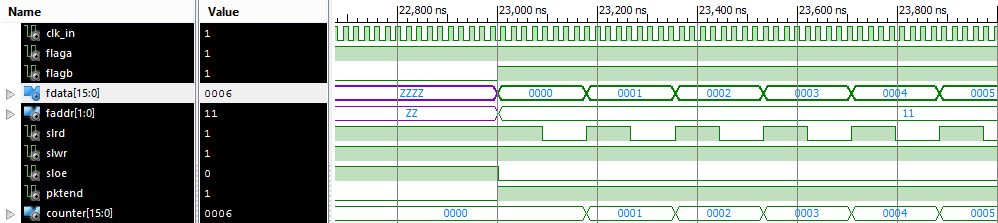
\includegraphics[height=.14\textheight]{sist_tb_lect.png}
		\caption{Simulación del inicio del ciclo de lectura}
		\label{test:tb:lect}
	\end{figure}

	La Figura \ref{test:tb:lect} muestra el diagrama temporal entregado por el simulador en donde se detalla el inicio de la operación de lectura de la memoria de la interfaz USB. Cuando la señal \textit{FLAGB} se encuentra en alto, el sistema activa la memoria FIFO del controlador FX2LP con dirección $''00''$ y habilita también su salida a través de la señal \textit{SLOE}. Luego, procede a leer la memoria colocando en bajo la señal \textit{SLRD}.
	
	Una vez leído el dato, se simula un cambio en la memoria a través del incremento en el contador y se lee el dato siguiente a través del flanco descendente de la señal \textit{SLRD}.
	
	\begin{figure}[b]
		\centering
		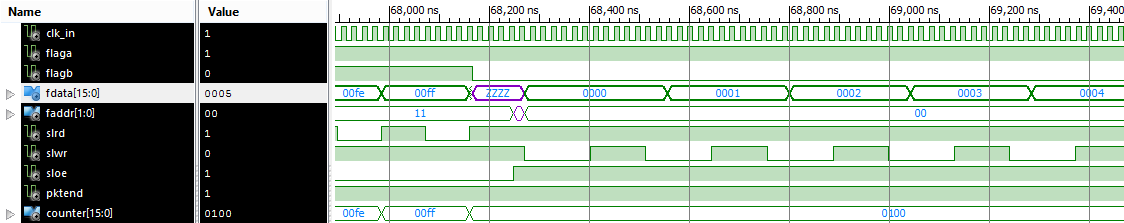
\includegraphics[height=.14\textheight]{sist_tb_esc}
		\caption{Simulación del inicio del ciclo de escritura}
		\label{test:tb:escr}
	\end{figure}

	Cuando fueron leídos todos los datos contenidos en el controlador FX2LP, este colocara en bajo la señal \textit{FLAGB}. Con esta señal,
	el FPGA comenzará el ciclo de escritura, reenviando los datos almacenados en su memoria. En la Figura \ref{test:tb:escr} se puede observar que cuando baja la señal, se interrumpe el ciclo de lectura y el sistema vuelve al de reset, para seguidamente iniciar el ciclo de escritura.
	
	Durante la operación de escritura, el bus \textit{FADDR[1:0]} es colocado en $''11'$ indicando la memoria FIFO receptora de los datos. Luego, activa y desactiva, en forma intermitente la señal \textit{SLWR}, enviando los datos almacenados en la memoria del FPGA hacia la memoria de la interfaz.
	
	\begin{figure}[t]
		\centering
		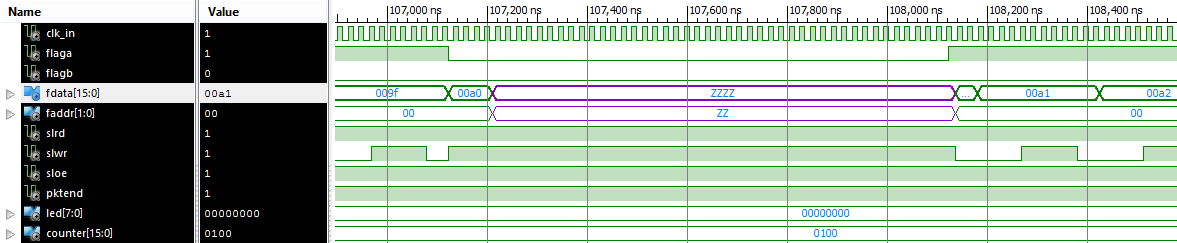
\includegraphics[height=.14\textheight]{sist_tb_esc_int}
		\caption{Simulación de una interrupción en el ciclo de escritura por falta de espacio en la memoria de la interfaz USB}
		\label{test:tb:int}
	\end{figure}
	
	Si por algún motivo la memoria de la interfaz USB se queda sin más espacio para el almacenamiento de los datos que provienen del FPGA, el controlador FX2LP coloca en bajo la señal \textit{FLAGA}. En la Figura \ref{test:tb:int} se observa que cuando baja la señal \textit{FLAGA}, el FPGA interrumpe el envío. Una vez que \textit{FLAGA} es nuevamente alta, la memoria sigue enviando los datos almacenados.
	
	\begin{figure}[b]
		\centering
		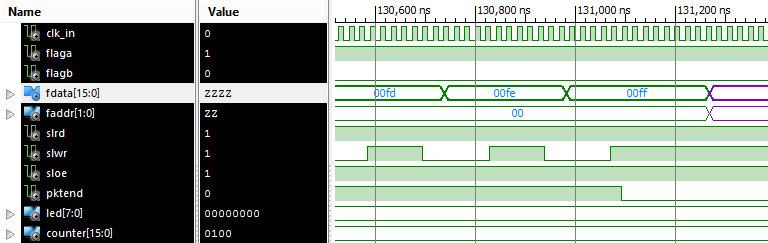
\includegraphics[height=.14\textheight]{sist_tb_pktend.png}
		\caption{Final de la simulación}
		\label{test:tb:pktend}
	\end{figure}

	Una vez que la memoria interna del FPGA se quedó sin datos, activa la señal PKTEND, indicando que terminó el envío de datos. Esto se puede observar en la Figura \ref{test:tb:pktend}. En ella se sabe que los datos de la memoria se acabaron debido a que el bus de datos alcanzó el mismo valor que el contador utilizado para emular el envío de datos desde la interfaz FX2LP.
	
	Luego de realizada la simulación y verificado que el funcionamiento del sistema es el esperado, se está en condiciones de cargar la síntesis del circuito en el FPGA.
	
\subsection{Carga del sistema de pruebas en el FPGA}
	Para efectuar la carga del sistema fue necesario especificar en el entorno de desarrollo ISE provisto por la compañía Xilinx Inc, en qué pines del FPGA debe asignar cada uno de los puertos descriptos en el código del sistema.
	
	Para indicarle al programa ISE dónde debe colocar los puertos se escribe un archivo denominado \textit{User Constraints File} (que significa Archivo de Restricciones del Usuario) y lleva como extensión la sigla \textit{ucf}.
	
	El archivo \textit{ufc} se generó a través de una interfaz gráfica provista por Xilinx Inc., denominada \textit{Plan Ahead}. En ella se puede cargar en una planilla la equivalencia entre los pines y los puertos, como así también los niveles de tensión lógicos necesarios.
	
	En la planilla se cargaron los puertos como se indican en la Tabla \ref{tab:fpga:conexion}. Con respecto a los niveles de tensión, se especificó que el estándar LVTTL, que es el especificado tanto en la placa Mojo v3\cite{Mojo}, como en el controlador FX2LP\cite{Cypress2017}. 
	
	También se especificó en el archivo \textit{ucf} la frecuencia de la entrada de reloj. Con esto, a la hora de generar el ruteo del FPGA, puede hacer un chequeo e informar si existe algún problema temporal en la implementación.
	
	Finalmente, se ejecutó el compilador para ejecutar el archivo que fue cargado en la memoria Flash de la placa de desarrollo Mojo v3 constatando que no existían errores.
	
	El texto completo del archivo \textit{ucf} generado, se observa en el Apéndice \ref{ap:vhdl}.